% Reset figure counter for this chapter to ensure consecutive numbering
\setcounter{figure}{0}

\section{External interface requirements}
\label{sec:external_interface_requirements}%

\subsection{User Interfaces}
\label{subsec:User_interfaces}%

Registered and non-registered users can access the Best Bike Paths (BBP) platform's \textbf{user interface} via a \textbf{mobile application} on any device with a current mobile operating system (iOS or Android) and an internet connection. The application is designed exclusively for mobile devices, providing an intuitive touch-based interface optimized for smartphones.

\subsubsection{Main User Interface}
\begin{enumerate}
    \item \textbf{Dashboard Overview:} Features fast buttons to previous ratings, paths and allows starting a new trip. The main screen provides quick access to all key features of the application. If the user is not registered, the buttons will lead to the registration form.
    \item \textbf{Trip Recording:} Interface for manual trip entry.
    \item \textbf{Path Search:} Search and visualize nearby bike paths or between origin and destination points.
    \item \textbf{Ratings and Reviews:} View and manage personal ratings and reviews of bike paths.
    \item \textbf{Path history:} Access to recent biking trips and their data.
    \item \textbf{Profile information:} Access to the profile and user information.
\end{enumerate}

\begin{figure}[H]
    \begin{center}
        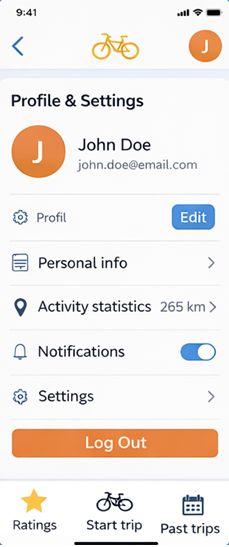
\includegraphics[width=0.35\linewidth, keepaspectratio=true]{Images/UI/profile.png}
        \caption{Profile settings and statistics screen.}
        \label{fig:profile_ui}%
    \end{center}
\end{figure}

\begin{figure}[H]
    \begin{center}
        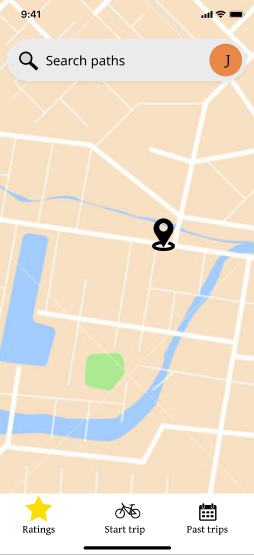
\includegraphics[width=0.35\linewidth, keepaspectratio=true]{Images/UI/main.png}
        \caption{Main App Interface}
        \label{fig:main_ui}%
    \end{center}
\end{figure}

\begin{figure}[H]
    \begin{center}
        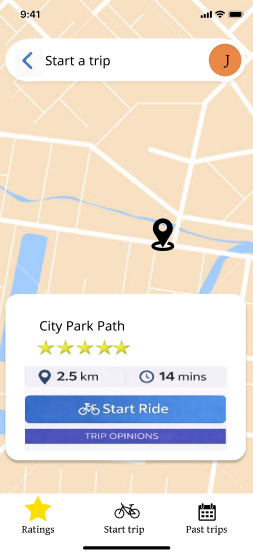
\includegraphics[width=0.35\linewidth, keepaspectratio=true]{Images/UI/start_trip.png}
        \caption{Interface when selecting a new path.}
        \label{fig:start_trip_ui}%
    \end{center}
\end{figure}

\begin{figure}[H]
    \begin{center}
        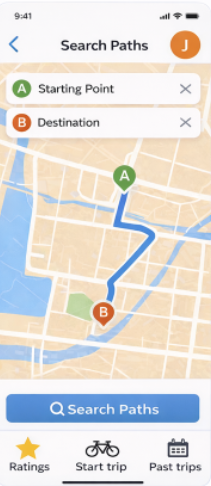
\includegraphics[width=0.35\linewidth, keepaspectratio=true]{Images/UI/search_paths.png}
        \caption{Interface for path searching in a certain area.}
        \label{fig:search_paths_ui}%
    \end{center}
\end{figure}

\subsubsection{Trips and reviews interface}
\begin{enumerate}
    \item The following screens show listings of trips and reviews.
    \item To retrieve more information about any of them, the user can click on each individual box and see information about it.
\end{enumerate}

\begin{figure}[H]
    \begin{center}
        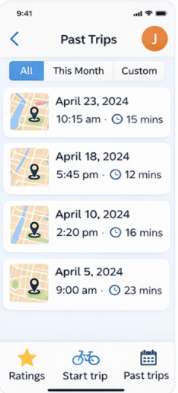
\includegraphics[width=0.35\linewidth, keepaspectratio=true]{Images/UI/past_trips.png}
        \caption{Past trips list.}
        \label{fig:past_trips_ui}%
    \end{center}
\end{figure}

\begin{figure}[H]
    \begin{center}
        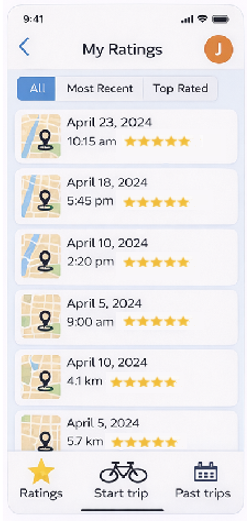
\includegraphics[width=0.35\linewidth, keepaspectratio=true]{Images/UI/my_ratings.png}
        \caption{List of the user ratingsl.}
        \label{fig:my_ratings_ui}%
    \end{center}
\end{figure}

\begin{figure}[H]
    \begin{center}
        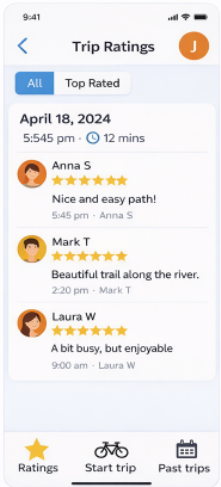
\includegraphics[width=0.35\linewidth, keepaspectratio=true]{Images/UI/trip_ratings.png}
        \caption{Interface for ratings of a certain path}
        \label{fig:trip_ratings_ui}%
    \end{center}
\end{figure}

\subsection{Hardware Interfaces}
\label{subsec:hardware_interfaces}%

The application is a mobile application compatible with mobile devices running iOS (version 13.0 or later) and Android (version 8.0 or later), with minimum screen resolution: 720x1280 pixels for optimal display. It requires a working GPS receiver, an accelerometer and a gyroscope for tracking and detection during the trips, and internet connectivity is required for logging in, loading and downloading the map, path information and reviews, and enough storage space for those files.

\subsection{Software Interfaces}
\label{subsec:software_interfaces}%

The system integrates a DBMS for trip information queries and user data retrieval. An Authentication system is required for user management and a file storage system for user generated content. 


\subsection{Communication Interfaces}
\label{subsec:communication_interfaces}%

The system uses JSON Data Format for data exchange between components. Node.js is used for connecting Backend and frontend. Push notifications are implemented for real-time user alerts. Email service integration is used for account management and notifications. DBMS connections are established using appropriate database software for data persistence and retrieval. External API integrations are implemented for weather services and map providers.

\section{Functional Requirements}
\label{sec:functional_requirements}%

\subsection{Requirements Lists}
\label{subsec:requirements3}%
\newcounter{req}
\setcounter{req}{1}
\newcommand{\creq}{\thereq\stepcounter{req}}

% Functional Requirements for F1
\subsubsection{F1. User Management}
\begin{center}
    \begin{longtable}{ |l|p{0.9\linewidth}| }
        \hline
        \textbf{ID} & \textbf{Description} \\
        \hline
        F1.1 & The system should enable users to create accounts using validated email addresses to access main functionalities.\\
        \hline
        F1.2 & The system should offer secure login mechanisms protected by passwords. \\
        \hline
        F1.3 & The system should permit users to modify their profile data, including contact information and personal preferences. \\
        \hline
        F1.4 & The system should include a password recovery feature that requires email confirmation. \\
        \hline
    \end{longtable}
\end{center}


% Functional Requirements for F2
\subsubsection{F2. Trip Recording}
\begin{center}
    \begin{longtable}{ |l|p{0.9\linewidth}| }
        \hline
        \textbf{ID} & \textbf{Description} \\
        \hline
        F2.1 & The system should allow registered users to manually record their cycling trips. \\
        \hline
        F2.2 & The system should automatically detect when a user is cycling based on speed analysis. \\
        \hline
        F2.3 & The system should collect GPS information to reconstruct the followed path during automatic trip recording. \\
        \hline
        F2.4 & The system should store trip data including start time, end time, duration, and route information. \\
        \hline
        F2.5 & The system should calculate trip statistics including total distance, average speed, and elevation changes. \\
        \hline
        F2.6 & The system should retrieve and integrate meteorological information from external services when available. \\
        \hline
        F2.7 & The system should allow users to view and manage their recorded trips. \\
        \hline
    \end{longtable}
\end{center}

% Functional Requirements for F3
\subsubsection{F3. Path Information Management}
\begin{center}
    \begin{longtable}{ |l|p{0.9\linewidth}| }
        \hline
        \textbf{ID} & \textbf{Description} \\
        \hline
        F3.1 & The system should allow registered users to manually insert bike path information including street names and path status. \\
        \hline
        F3.2 & The system should allow registered users to specify path status (e.g., optimal, medium, sufficient, requires maintenance). \\
        \hline
        F3.3 & The system should allow registered users to mark obstacles such as potholes on paths. \\
        \hline
        F3.4 & The system should allow registered users to make path information publishable. \\
        \hline
        F3.5 & The system should store path information including origin, destination, status, and associated obstacles. \\
        \hline
        F3.6 & The system should track the freshness of path information (required for merging functionality). \\
        \hline
    \end{longtable}
\end{center}

% Functional Requirements for F4
\subsubsection{F4. Automated Path Detection}
\begin{center}
    \begin{longtable}{ |l|p{0.9\linewidth}| }
        \hline
        \textbf{ID} & \textbf{Description} \\
        \hline
        F4.1 & The system should automatically detect when a user is biking based on speed analysis from mobile device sensors. \\
        \hline
        F4.2 & The system should collect GPS information during automatic trip recording to reconstruct the followed path. \\
        \hline
        F4.3 & The system should acquire data from mobile device accelerometer and gyroscope to detect device movements suggesting potholes or other obstacles. \\
        \hline
        F4.4 & The system should present automatically detected paths and obstacles to the user for confirmation or correction. \\
        \hline
        F4.5 & The system should allow users to confirm automatically detected information before making it available to the community (Avoid false positives) \\
        \hline
        F4.6 & The system should allow users to correct false positives in automatically detected obstacles. \\
        \hline
        F4.7 & The system should store confirmed path and obstacle information after user validation. \\
        \hline
    \end{longtable}
\end{center}

% Functional Requirements for F5
\subsubsection{F5. Path Search and Visualization}
\begin{center}
    \begin{longtable}{ |l|p{0.9\linewidth}| }
        \hline
        \textbf{ID} & \textbf{Description} \\
        \hline
        F5.1 & The system should allow all users (registered and non-registered) to specify an origin and destination. \\
        \hline
        F5.2 & The system should find all available bike paths between the specified origin and destination. \\
        \hline
        F5.3 & The system should compute a score for each path based on path status and effectiveness in reaching the destination. \\
        \hline
        F5.4 & The system should visualize paths on a map ranked by their computed scores. \\
        \hline
    \end{longtable}
\end{center}

% Functional Requirements for F6
\subsubsection{F6. Information Merging}
\begin{center}
    \begin{longtable}{ |l|p{0.9\linewidth}| }
        \hline
        \textbf{ID} & \textbf{Description} \\
        \hline
        F6.1 & The system should collect publishable information about paths from multiple users. \\
        \hline
        F6.2 & The system should merge different pieces of information considering their freshness. \\
        \hline
        F6.3 & The system should merge different pieces of information considering the number of confirming data obtained. \\
        \hline
        F6.4 & The system should resolve conflicts when multiple users provide conflicting path status information. \\
        \hline
        F6.5 & The system should prioritize information based on recency and consensus. \\
        \hline
    \end{longtable}
\end{center}

\subsection{Dependencies}
\label{subsec:dependencies}%

\subsubsection{F1 Dependencies}
\begin{itemize}
    \item \textbf{F1.1:} Must be completed before any other functionality requiring registered users.
    \item \textbf{F1.2:} Is required for all registered user operations.
\end{itemize}

\subsubsection{F2 Dependencies}
\begin{itemize}
    \item Requires F1 completion.
    \item \textbf{F2.2:} Must be completed before F4.1.
    \item \textbf{F2.6:} Requires external weather API integration.
\end{itemize}

\subsubsection{F3 Dependencies}
\begin{itemize}
    \item Requires F1 completion.
    \item \textbf{F3.1:} Must be completed before F3.4.
    \item \textbf{F3.6:} Is required for F6.2.
\end{itemize}

\subsubsection{F4 Dependencies}
\begin{itemize}
    \item Requires F1 and F2 completion.
    \item \textbf{F4.1:} Must be completed before F4.2 and F4.3.
    \item \textbf{F4.5:} Must be completed before F4.6.
    \item \textbf{F4.7:} Feeds into F6.1.
\end{itemize}

\subsubsection{F5 Dependencies}
\begin{itemize}
    \item Requires F3 completion.
    \item \textbf{F5.1:} Must be completed before F5.2.
    \item \textbf{F5.3:} Requires F3.2 and F3.6 completion.
    \item Requires map service API integration.
\end{itemize}

\subsubsection{F6 Dependencies}
\begin{itemize}
    \item Requires F3 and F4 completion.
    \item \textbf{F6.1:} Must be completed before F6.2 and F6.3.
    \item \textbf{F6.4:} Requires F6.2 and F6.3 completion.
\end{itemize}

\subsection{Requirement Priorities and Implementation Focus}
\label{subsec:priority_criticality_matrix}%

Functional requirements are classified into three implementation phases:

\textbf{Phase 1 - Critical Requirements (High Priority):} User Management (F1), Trip Recording (F2), Path Information Management (F3), and Path Search and Visualization (F5). These form the core foundation of the system.

\textbf{Phase 2 - Important Requirements (Medium Priority):} Automated Path Detection (F4). This enhances user convenience but the system can function with manual recording.

\textbf{Phase 3 - Standard Requirements (Low Priority):} Information Merging (F6). This optimizes data quality but is not essential for basic operation.

\newpage
\subsection{Use case diagrams}
\label{subsec:use_case_diagrams}%

% Reset figure counter to ensure consecutive numbering starting from this section
\setcounter{figure}{0}

\begin{figure}[H]
    \begin{center}
        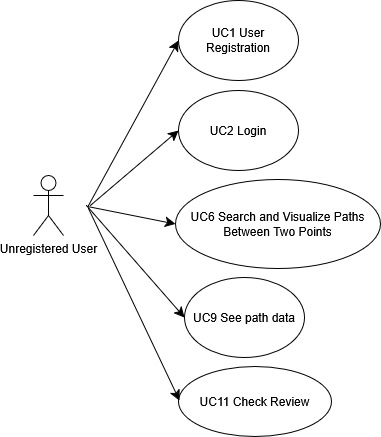
\includegraphics[width=0.75\linewidth, keepaspectratio=true]{Images/Diagrams/UseCase_NonRegistered.jpeg}
        \caption{Use Cases Diagram for Non-Registered Users.} 
        \label{fig:NonRegisteredUC}%
    \end{center}
\end{figure}



\begin{figure}[H]
    \begin{center}
        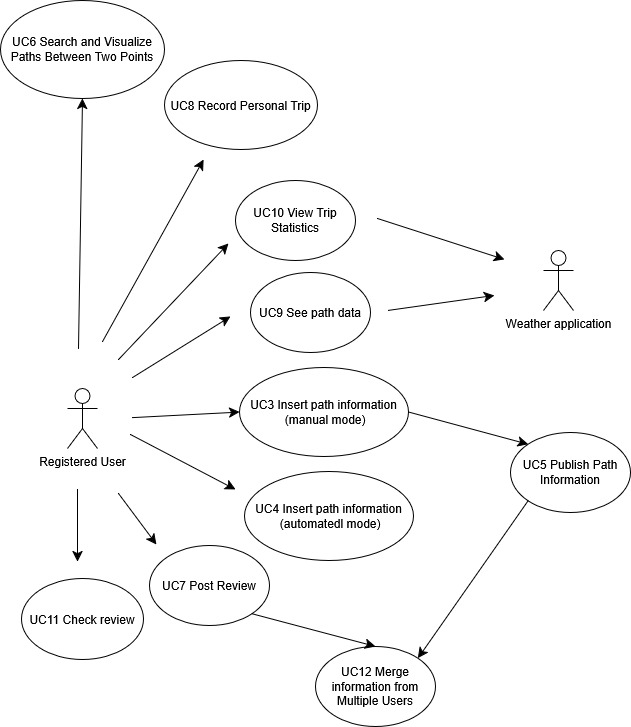
\includegraphics[width=0.8\linewidth, keepaspectratio=true]{Images/Diagrams/UseCase_Registered.jpeg}
        \caption{Use Cases Diagram for Registered Users}
        \label{fig:RegisteredUC}%
    \end{center}
\end{figure}

\subsection{Use cases}
\label{subsec:use_cases}%
\newcounter{uc}
\setcounter{uc}{1}
\newcommand{\cuc}{\theuc\stepcounter{uc}}
The primary identified use cases are described and illustrated in this section.
Each of them has a table with \textbf{entry conditions, event flow, exit conditions, and exceptions, as well as a sequence diagram} that displays the messages sent back and forth between the called functions and the entities.

% Reset table counter to ensure consecutive numbering starting from this section
\setcounter{table}{0}

\subsubsection*{UC\cuc . User Registration}
\begin{center}
    \begin{longtable}{|l|p{0.75\linewidth}|}
        \hline
        \textbf{Actor}            & User, Email Provider \\
        \hline
        \textbf{Entry Conditions} & 
        \begin{itemize}
            \item User not registered in BBP
            \item User has valid email address
            \item User meets platform requirements
        \end{itemize} \\
        \hline
        \textbf{Event Flow}       & 
        \begin{enumerate}
            \item BBP shows the login form with registration option
            \item User clicks on "Create Account"
            \item BBP displays registration form
            \item User enters information:
            \begin{itemize}
                \item Username
                \item Email address
                \item Password
                \item Confirm password
            \end{itemize}
            \item BBP validates user information
            \item BBP checks if email is already registered
            \item BBP sends verification email
            \item User clicks verification link in email
            \item BBP activates user account
            \item BBP redirects user to login page
        \end{enumerate} \\
        \hline
        \textbf{Exit Conditions}   & 
        \begin{itemize}
            \item User account is created and verified
            \item User can access the system
        \end{itemize} \\
        \hline
        \textbf{Exceptions}       & 
        \begin{enumerate}
            \item \textbf{Email already registered:}
            \begin{itemize}
                \item Show existing account message
                \item Provide login option or password recovery
            \end{itemize}
            \item \textbf{Invalid email format:}
            \begin{itemize}
                \item Request valid email address
                \item Highlight email field error
            \end{itemize}
            \item \textbf{Weak password:}
            \begin{itemize}
                \item Show password requirements
                \item Request stronger password
            \end{itemize}
            \item \textbf{Email verification timeout:}
            \begin{itemize}
                \item Allow resending verification email
                \item Provide support contact
            \end{itemize}
        \end{enumerate} \\
        \hline
        \caption{User Registration Use Case.}
        \label{tab:user_registration_use_case}
    \end{longtable}
\end{center}

\begin{figure}[H]
    \begin{center}
        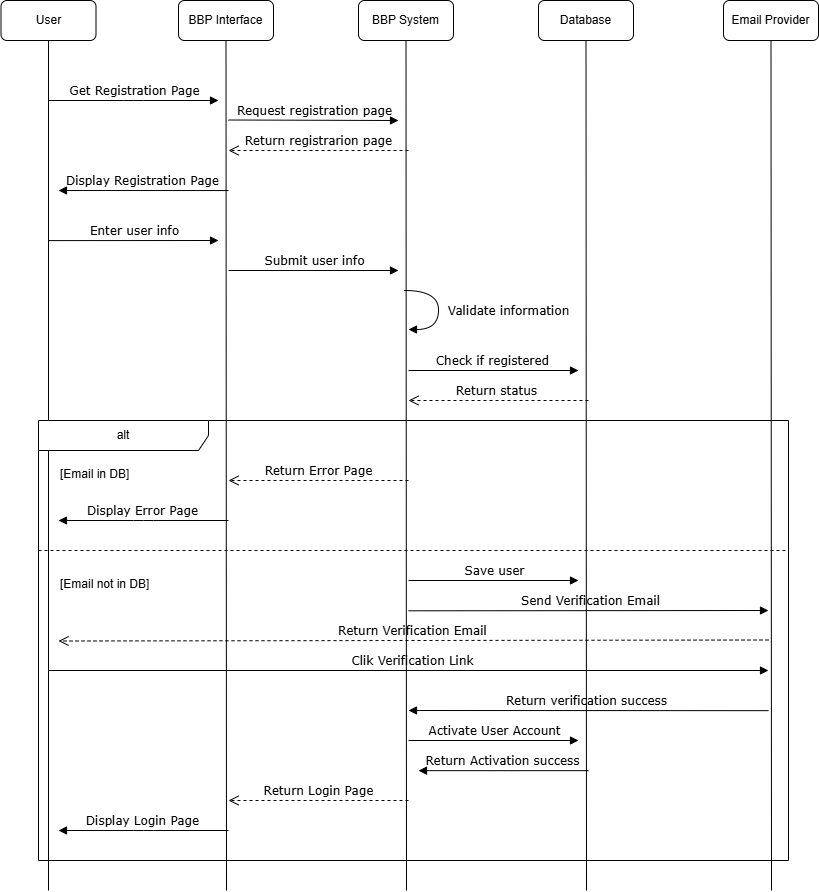
\includegraphics[width=1.15\linewidth, height=\paperheight, keepaspectratio=true]{Images/Diagrams/Sequence_UserRegistration.png}
        \caption{Sequence Diagram for User Registration}
        \label{fig:user_registration_seqd}%
    \end{center}
\end{figure}

\subsubsection*{UC\cuc . Login}
\begin{center}
    \begin{longtable}{|l|p{0.75\linewidth}|}
        \hline
        \textbf{Actor}            & Registered User \\
        \hline
        \textbf{Entry Conditions} & 
        \begin{itemize}
            \item User has a registered account
            \item User account is verified and active
        \end{itemize} \\
        \hline
        \textbf{Event Flow}       & 
        \begin{enumerate}
            \item BBP displays login screen
            \item User enters credentials:
            \begin{itemize}
                \item Username or email address
                \item Password
            \end{itemize}
            \item BBP validates credentials
            \item BBP verifies account is active
            \item BBP creates user session
            \item BBP redirects user to main dashboard
        \end{enumerate} \\
        \hline
        \textbf{Exit Conditions}   & 
        \begin{itemize}
            \item User is authenticated and logged in
            \item User session is established
            \item User can access registered user features
        \end{itemize} \\
        \hline
        \textbf{Exceptions}       & 
        \begin{enumerate}
            \item \textbf{Invalid credentials:}
            \begin{itemize}
                \item Display error message
                \item Provide password recovery option
            \end{itemize}
            \item \textbf{Account not verified:}
            \begin{itemize}
                \item Prompt user to verify email
                \item Offer option to resend verification email
            \end{itemize}
            \item \textbf{Account suspended or inactive:}
            \begin{itemize}
                \item Display account status message
                \item Provide contact support option
            \end{itemize}
            \item \textbf{Network error:}
            \begin{itemize}
                \item Display connection error
                \item Provide retry option
            \end{itemize}
        \end{enumerate} \\
        \hline
        \caption{Login Use Case.}
        \label{tab:login_use_case}
    \end{longtable}
\end{center}

\begin{figure}[H]
    \begin{center}
        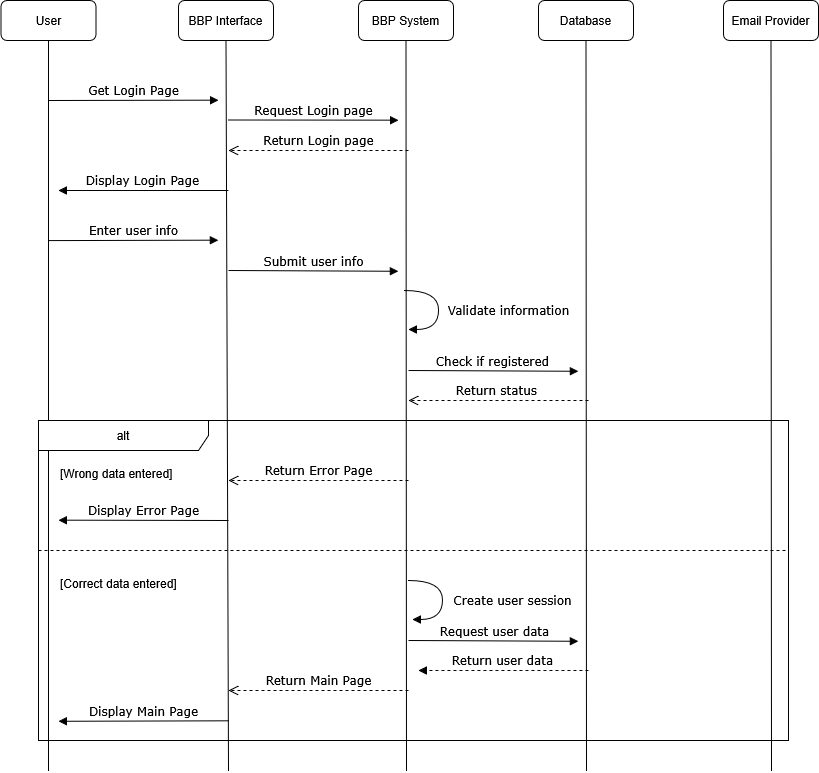
\includegraphics[width=1\linewidth]{Images/Diagrams/Sequence_Login.png}
        \caption{Sequence Diagram for Login}
        \label{fig:login_seqd}%
    \end{center}
\end{figure}

\subsubsection*{UC\cuc . Insert Path Information (Manual Mode)}
\begin{center}
    \begin{longtable}{|l|p{0.75\linewidth}|}
        \hline
        \textbf{Actor}            & Registered User \\
        \hline
        \textbf{Entry Conditions} & 
        \begin{itemize}
            \item User is logged in
            \item User has knowledge of a bike path
        \end{itemize} \\
        \hline
        \textbf{Event Flow}       & 
        \begin{enumerate}
            \item User accesses path management interface
            \item User selects "Add New Path"
            \item BBP displays path creation form
            \item User enters path information:
            \begin{itemize}
                \item Path name
                \item Street names in the path
                \item Origin location
                \item Destination location
                \item Path status (optimal, medium, sufficient, requires maintenance)
            \end{itemize}
            \item User optionally marks obstacles:
            \begin{itemize}
                \item Pothole locations
                \item Other obstacles
            \end{itemize}
            \item BBP validates path information
            \item BBP checks for duplicate paths
            \item User chooses to make path publishable or keep it private
            \item BBP saves path information
            \item BBP displays confirmation message
        \end{enumerate} \\
        \hline
        \textbf{Exit Conditions}   & 
        \begin{itemize}
            \item Path information is saved
            \item Path is available for user's personal use or published to community
        \end{itemize} \\
        \hline
        \textbf{Exceptions}       & 
        \begin{enumerate}
            \item \textbf{Incomplete required fields:}
            \begin{itemize}
                \item Highlight missing fields
                \item Save as draft
            \end{itemize}
            \item \textbf{Duplicate path detected:}
            \begin{itemize}
                \item Show existing path
                \item Offer update option
            \end{itemize}
            \item \textbf{Invalid location data:}
            \begin{itemize}
                \item Request valid location information
                \item Provide map selection tool
            \end{itemize}
            \item \textbf{Network error:}
            \begin{itemize}
                \item Save path data locally
                \item Sync when connection is restored
            \end{itemize}
        \end{enumerate} \\
        \hline
        \caption{Insert Path Information (Manual Mode) Use Case.}
        \label{tab:insert_path_manual_use_case}
    \end{longtable}
\end{center}

\begin{figure}[H]
    \raggedright
    \hspace*{-2cm}
    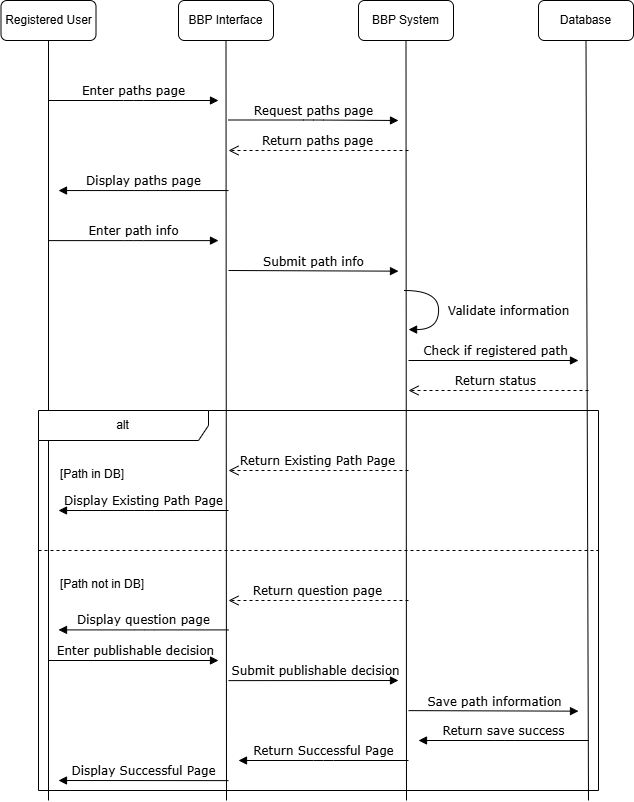
\includegraphics[width=1.1\linewidth]{Images/Diagrams/Sequence_InsertPathManual.png}
    \caption{Sequence Diagram for Insert Path Information (Manual Mode)}
    \label{fig:insert_path_manual_seqd}%
\end{figure}

\subsubsection*{UC\cuc . Insert Path Information (Automated Mode)}
\begin{center}
    \begin{longtable}{|l|p{0.75\linewidth}|}
        \hline
        \textbf{Actor}            & Registered User, Mobile Device Sensors \\
        \hline
        \textbf{Entry Conditions} & 
        \begin{itemize}
            \item User is logged in
            \item User has enabled automatic trip detection
            \item Mobile device has GPS and sensor access granted
            \item User is cycling
        \end{itemize} \\
        \hline
        \textbf{Event Flow}       & 
        \begin{enumerate}
            \item BBP monitors user's speed from GPS data
            \item BBP detects cycling speed pattern
            \item BBP begins automatic trip recording:
            \begin{itemize}
                \item Collects GPS coordinates continuously
                \item Monitors accelerometer for significant movements
                \item Monitors gyroscope for device movements
            \end{itemize}
            \item BBP detects potential obstacles:
            \begin{itemize}
                \item Analyzes accelerometer data for pothole-like patterns
                \item Records location of detected anomalies
            \end{itemize}
            \item User finishes cycling trip
            \item BBP stops recording
            \item BBP reconstructs path from collected GPS data
            \item BBP displays detected path and obstacles to the user
            \item User reviews detected path information:
            \begin{itemize}
                \item Verifies route accuracy
                \item Confirms origin and destination
            \end{itemize}
            \item User reviews detected obstacles:
            \begin{itemize}
                \item Confirms true positives
                \item Dismisses false positives
            \end{itemize}
            \item User corrects detected information if necessary:
            \begin{itemize}
                \item Adjusts path route
                \item Modifies obstacle locations
                \item Adds missed obstacles
            \end{itemize}
            \item User confirms final path information
            \item BBP validates and saves confirmed path information
            \item User chooses to make path publishable or keep it private
            \item BBP updates path database and confirms completion
        \end{enumerate} \\
        \hline
        \textbf{Exit Conditions}   & 
        \begin{itemize}
            \item Path is automatically detected and recorded
            \item User has confirmed or corrected detected information
            \item Path is available for user's personal use or published to community
        \end{itemize} \\
        \hline
        \textbf{Exceptions}       & 
        \begin{enumerate}
            \item \textbf{GPS signal lost:}
            \begin{itemize}
                \item Continue recording with available data
                \item Notify user of signal loss
            \end{itemize}
            \item \textbf{Sensor data unavailable:}
            \begin{itemize}
                \item Record path without obstacle detection
                \item Notify user of sensor limitations
            \end{itemize}
            \item \textbf{False positive obstacles:}
            \begin{itemize}
                \item User dismisses false detections
                \item System learns from corrections
            \end{itemize}
            \item \textbf{User cancels recording:}
            \begin{itemize}
                \item Discard recorded data
                \item Return to previous state
            \end{itemize}
            \item \textbf{Battery low:}
            \begin{itemize}
                \item Save current progress
                \item Notify user to charge device
            \end{itemize}
            \item \textbf{Network error during save:}
            \begin{itemize}
                \item Save confirmed data locally
                \item Synchronize when connection is restored
            \end{itemize}
        \end{enumerate} \\
        \hline
        \caption{Insert Path Information (Automated Mode) Use Case.}
        \label{tab:insert_path_automated_use_case}
    \end{longtable}
\end{center}

\begin{figure}[H]
    \begin{center}
        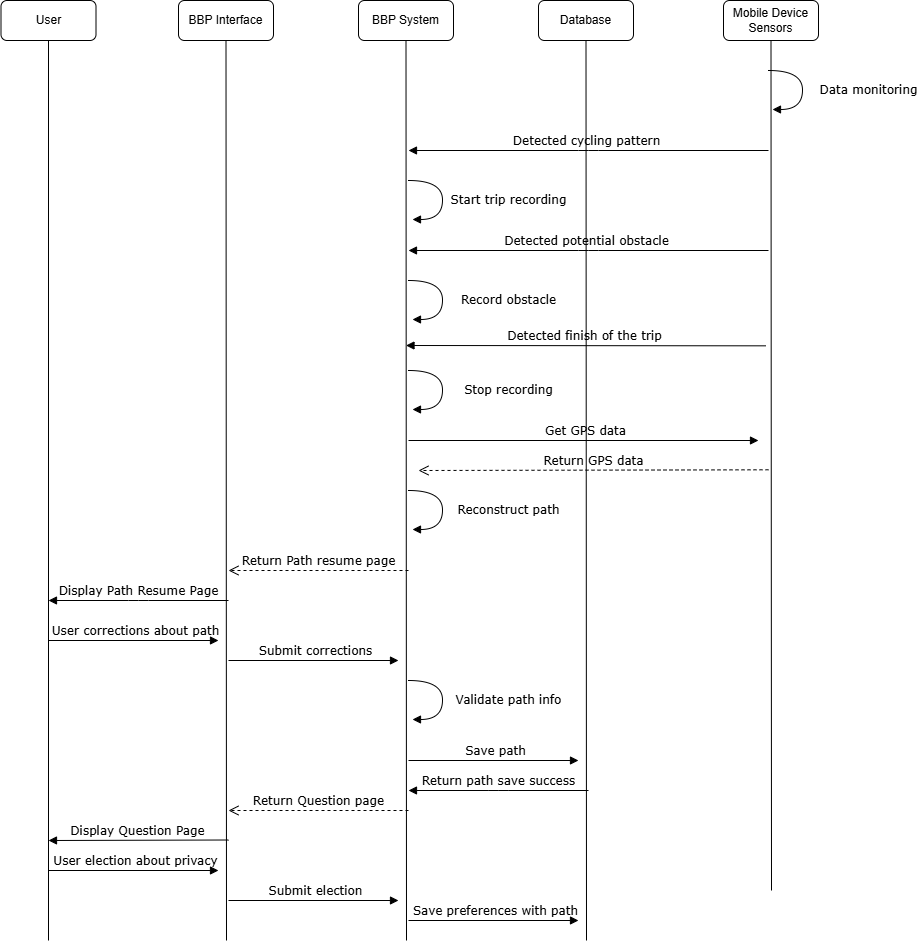
\includegraphics[width=1\linewidth]{Images/Diagrams/Sequence_InsertPathAutomated.png}
        \caption{Sequence Diagram for Insert Path Information (Automated Mode)}
        \label{fig:insert_path_automated_seqd}%
    \end{center}
\end{figure}

\subsubsection*{UC\cuc . Publish Path Information}
\begin{center}
    \begin{longtable}{|l|p{0.75\linewidth}|}
        \hline
        \textbf{Actor}            & Registered User \\
        \hline
        \textbf{Entry Conditions} & 
        \begin{itemize}
            \item User is logged in
            \item User has created or recorded a path
            \item Path information is complete
        \end{itemize} \\
        \hline
        \textbf{Event Flow}       & 
        \begin{enumerate}
            \item User accesses path management interface
            \item User selects a path from their saved paths
            \item User views path details
            \item User selects "Publish Path" option
            \item BBP displays publication confirmation dialog
            \item User confirms publication
            \item BBP validates path information completeness
            \item BBP changes path status to published
            \item BBP makes path available to all users
            \item BBP displays confirmation message
            \item Path appears in public path database
        \end{enumerate} \\
        \hline
        \textbf{Exit Conditions}   & 
        \begin{itemize}
            \item Path is published and available to all users
            \item Path appears in search results
        \end{itemize} \\
        \hline
        \textbf{Exceptions}       & 
        \begin{enumerate}
            \item \textbf{Incomplete path information:}
            \begin{itemize}
                \item Highlight missing information
                \item Request completion before publishing
            \end{itemize}
            \item \textbf{Path already published:}
            \begin{itemize}
                \item Show current publication status
                \item Offer unpublish option
            \end{itemize}
            \item \textbf{Network error:}
            \begin{itemize}
                \item Save publication request locally
                \item Sync when connection is restored
            \end{itemize}
        \end{enumerate} \\
        \hline
        \caption{Publish Path Information Use Case.}
        \label{tab:publish_path_use_case}
    \end{longtable}
\end{center}

\begin{figure}[H]
    \begin{center}
        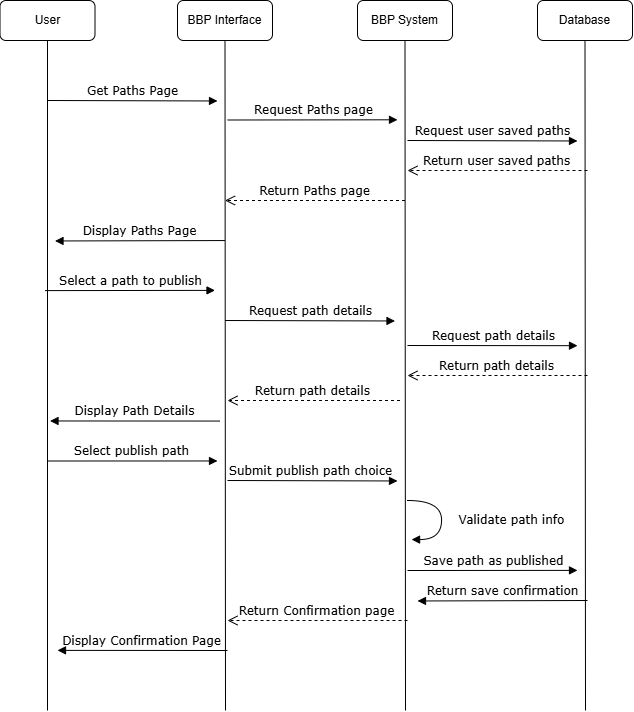
\includegraphics[width=1\linewidth]{Images/Diagrams/Sequence_PublishPath.png}
        \caption{Sequence Diagram for Publish Path Information}
        \label{fig:publish_path_seqd}%
    \end{center}
\end{figure}

\subsubsection*{UC\cuc . Search and Visualize Paths Between Two Points}
\begin{center}
    \begin{longtable}{|l|p{0.75\linewidth}|}
        \hline
        \textbf{Actor}            & User (Registered or Non-Registered) \\
        \hline
        \textbf{Entry Conditions} & 
        \begin{itemize}
            \item User has access to BBP platform
            \item Published paths exist in the system
        \end{itemize} \\
        \hline
        \textbf{Event Flow}       & 
        \begin{enumerate}
            \item User accesses path search interface
            \item User specifies origin location
            \item User specifies destination location
            \item BBP validates location inputs
            \item BBP searches for all available paths between origin and destination
            \item BBP computes score for each path:
            \begin{itemize}
                \item Considers path status
                \item Considers path effectiveness
                \item Considers presence of obstacles
            \end{itemize}
            \item BBP ranks paths by computed score
            \item BBP displays paths on map visualization
            \item User can view details of each path:
            \begin{itemize}
                \item Path status
                \item Detected obstacles
                \item Path rating
                \item Distance
            \end{itemize}
            \item User can select a path to follow
        \end{enumerate} \\
        \hline
        \textbf{Exit Conditions}   & 
        \begin{itemize}
            \item User can see available paths between origin and destination
            \item Paths are ranked and visualized on map
            \item User can access path details
        \end{itemize} \\
        \hline
        \textbf{Exceptions}       & 
        \begin{enumerate}
            \item \textbf{No paths found:}
            \begin{itemize}
                \item Display message that no paths are available
                \item Suggest nearby paths or alternative destinations
            \end{itemize}
            \item \textbf{Invalid location:}
            \begin{itemize}
                \item Request valid location information
                \item Provide location selection assistance
            \end{itemize}
            \item \textbf{Map service unavailable:}
            \begin{itemize}
                \item Display path list without map visualization
                \item Notify user of map service issue
            \end{itemize}
            \item \textbf{Origin equals destination:}
            \begin{itemize}
                \item Display error message
                \item Request different locations
            \end{itemize}
        \end{enumerate} \\
        \hline
        \caption{Search and Visualize Paths Between Two Points Use Case.}
        \label{tab:search_paths_use_case}
    \end{longtable}
\end{center}

\begin{figure}[H]
    \begin{center}
        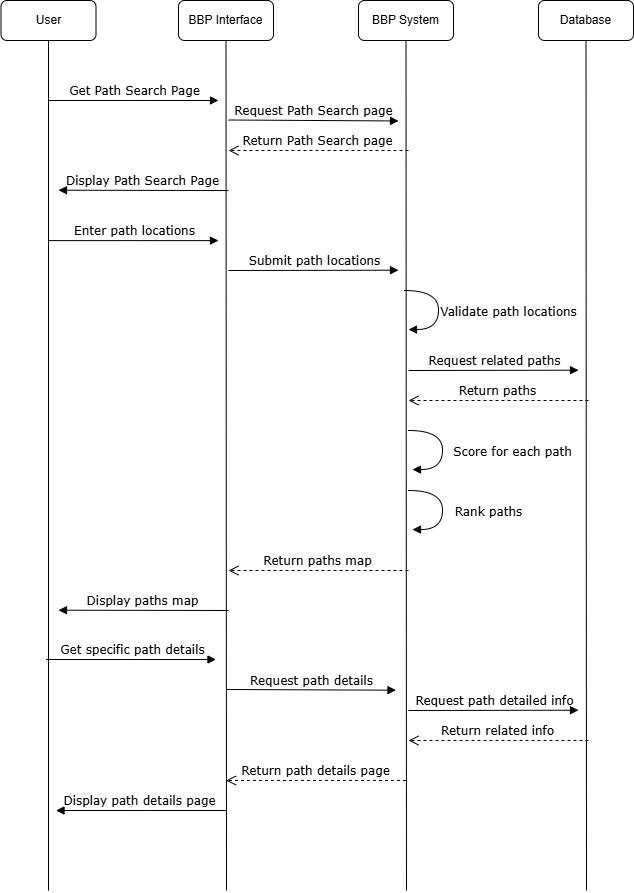
\includegraphics[width=1\linewidth]{Images/Diagrams/Sequence_SearchPaths.png}
        \caption{Sequence Diagram for Search and Visualize Paths Between Two Points}
        \label{fig:search_paths_seqd}%
    \end{center}
\end{figure}

\subsubsection*{UC\cuc . Post Review}
\begin{center}
    \begin{longtable}{|l|p{0.75\linewidth}|}
        \hline
        \textbf{Actor}            & Registered User \\
        \hline
        \textbf{Entry Conditions} & 
        \begin{itemize}
            \item User is logged in
            \item User has knowledge or experience with a specific path
            \item Path exists in the system (either published or user's own path)
        \end{itemize} \\
        \hline
        \textbf{Event Flow}       & 
        \begin{enumerate}
            \item User accesses path details interface
            \item User selects a path to review
            \item BBP displays path information and review option
            \item User selects "Add Review" or "Rate Path"
            \item BBP displays review form
            \item User enters review information:
            \begin{itemize}
                \item Rating (numerical score)
                \item Path status update (optional: optimal, medium, sufficient, requires maintenance)
                \item Written comment (optional)
                \item Date of experience
            \end{itemize}
            \item User submits review
            \item BBP validates review data
            \item BBP saves review to path
            \item BBP recalculates path's overall rating
            \item BBP updates path status if applicable
            \item BBP displays confirmation message
            \item Review appears in path's review list
        \end{enumerate} \\
        \hline
        \textbf{Exit Conditions}   & 
        \begin{itemize}
            \item Review is saved and associated with the path
            \item Path's overall rating is updated
            \item Review is visible to all users viewing the path
        \end{itemize} \\
        \hline
        \textbf{Exceptions}       & 
        \begin{enumerate}
            \item \textbf{Missing required fields:}
            \begin{itemize}
                \item Highlight missing fields
                \item Request completion before submission
            \end{itemize}
            \item \textbf{Duplicate review from same user on same day:}
            \begin{itemize}
                \item Show existing review
                \item Offer option to edit instead
            \end{itemize}
            \item \textbf{Network error:}
            \begin{itemize}
                \item Save review locally
                \item Sync when connection is restored
            \end{itemize}
            \item \textbf{Path no longer exists:}
            \begin{itemize}
                \item Display error message
                \item Return to path search
            \end{itemize}
        \end{enumerate} \\
        \hline
        \caption{Post Review Use Case.}
        \label{tab:post_review_use_case}
    \end{longtable}
\end{center}

\begin{figure}[H]
    \begin{center}
        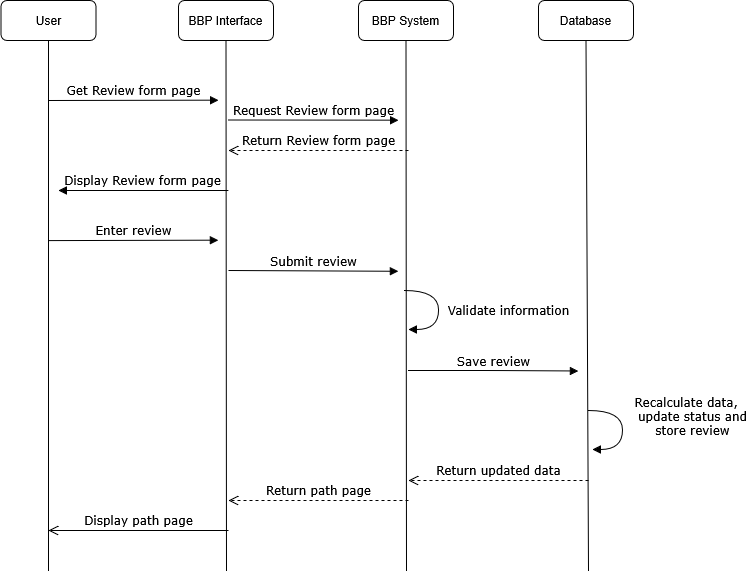
\includegraphics[width=1\linewidth]{Images/Diagrams/Sequence_PostReview.png}
        \caption{Sequence Diagram for Post Review}
        \label{fig:post_review_seqd}%
    \end{center}
\end{figure}

\subsubsection*{UC\cuc . Record Personal Trip}
\begin{center}
    \begin{longtable}{|l|p{0.75\linewidth}|}
        \hline
        \textbf{Actor}            & Registered User \\
        \hline
        \textbf{Entry Conditions} & 
        \begin{itemize}
            \item User is logged in
            \item User has completed a cycling trip
        \end{itemize} \\
        \hline
        \textbf{Event Flow}       & 
        \begin{enumerate}
            \item User accesses trip recording interface
            \item User selects "Record New Trip"
            \item BBP displays trip entry form
            \item User enters trip information:
            \begin{itemize}
                \item Start location
                \item End location
                \item Start time
                \item End time
                \item Route information (optional)
            \end{itemize}
            \item BBP validates trip data
            \item BBP calculates trip statistics:
            \begin{itemize}
                \item Total distance
                \item Average speed
                \item Duration
                \item Elevation changes (if available)
            \end{itemize}
            \item BBP retrieves weather information from external service (if available)
            \item BBP enriches trip data with meteorological information
            \item BBP saves trip to user's trip history
            \item BBP displays trip summary with statistics
        \end{enumerate} \\
        \hline
        \textbf{Exit Conditions}   & 
        \begin{itemize}
            \item Trip is recorded and saved
            \item Trip statistics are calculated and displayed
            \item Trip appears in user's trip history
        \end{itemize} \\
        \hline
        \textbf{Exceptions}       & 
        \begin{enumerate}
            \item \textbf{Invalid time range:}
            \begin{itemize}
                \item Show time validation error
                \item Request valid start and end times
            \end{itemize}
            \item \textbf{Weather service unavailable:}
            \begin{itemize}
                \item Save trip without weather data
                \item Notify user that weather data is unavailable
            \end{itemize}
            \item \textbf{Invalid location data:}
            \begin{itemize}
                \item Request valid location information
                \item Provide location selection assistance
            \end{itemize}
            \item \textbf{Network error:}
            \begin{itemize}
                \item Save trip data locally
                \item Sync when connection is restored
            \end{itemize}
        \end{enumerate} \\
        \hline
        \caption{Record Personal Trip Use Case.}
        \label{tab:record_personal_trip_use_case}
    \end{longtable}
\end{center}

\begin{figure}[H]
    \begin{center}
        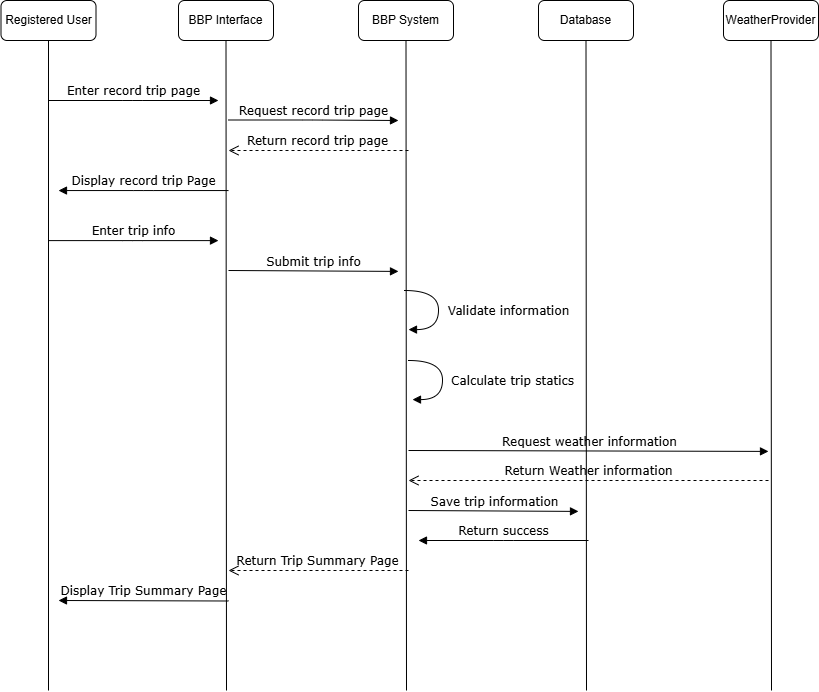
\includegraphics[width=1\linewidth]{Images/Diagrams/Sequence_RecordTrip.png}
        \caption{Sequence Diagram for Record Personal Trip}
        \label{fig:record_trip_seqd}%
    \end{center}
\end{figure}

\subsubsection*{UC\cuc . See Path Data}
\begin{center}
    \begin{longtable}{|l|p{0.75\linewidth}|}
        \hline
        \textbf{Actor}            & User (Registered or Non-Registered) \\
        \hline
        \textbf{Entry Conditions} & 
        \begin{itemize}
            \item User has access to BBP platform
            \item Path exists in the system
        \end{itemize} \\
        \hline
        \textbf{Event Flow}       & 
        \begin{enumerate}
            \item User accesses path browsing interface
            \item User searches for or selects a specific path
            \item BBP retrieves path information from database
            \item BBP displays comprehensive path data:
            \begin{itemize}
                \item Path name
                \item Origin and destination
                \item Street names
                \item Total distance
                \item Current status (optimal, medium, sufficient, requires maintenance)
                \item Overall rating
                \item Date last updated
            \end{itemize}
            \item BBP displays obstacle information:
            \begin{itemize}
                \item Pothole locations on map
                \item Other obstacles
                \item Date obstacles were reported
            \end{itemize}
            \item BBP displays reviews and comments from users
            \item BBP shows path route on map
            \item User can view additional details:
            \begin{itemize}
                \item Number of users who have used the path
                \item Statistics about the path
                \item Alternative similar paths
            \end{itemize}
        \end{enumerate} \\
        \hline
        \textbf{Exit Conditions}   & 
        \begin{itemize}
            \item User has viewed comprehensive path information
            \item User can make informed decision about using the path
        \end{itemize} \\
        \hline
        \textbf{Exceptions}       & 
        \begin{enumerate}
            \item \textbf{Path not found:}
            \begin{itemize}
                \item Display error message
                \item Suggest similar paths or return to search
            \end{itemize}
            \item \textbf{Incomplete path data:}
            \begin{itemize}
                \item Display available information
                \item Note missing data to user
            \end{itemize}
            \item \textbf{Map service unavailable:}
            \begin{itemize}
                \item Display path information without map
                \item Notify user of map service issue
            \end{itemize}
            \item \textbf{Network error:}
            \begin{itemize}
                \item Display cached data if available
                \item Notify user of connection issue
            \end{itemize}
        \end{enumerate} \\
        \hline
        \caption{See Path Data Use Case.}
        \label{tab:see_path_data_use_case}
    \end{longtable}
\end{center}

\begin{figure}[H]
    \begin{center}
        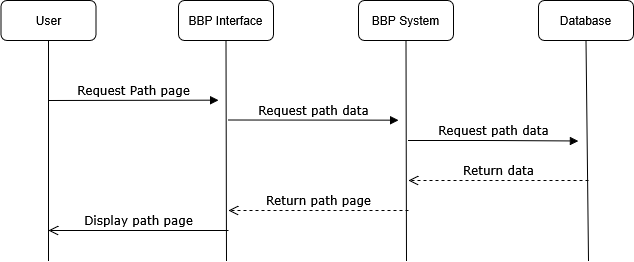
\includegraphics[width=1\linewidth]{Images/Diagrams/Sequence_SeePathData.png}
        \caption{Sequence Diagram for See Path Data}
        \label{fig:see_path_data_seqd}%
    \end{center}
\end{figure}

\subsubsection*{UC\cuc . View Trip Statistics}
\begin{center}
    \begin{longtable}{|l|p{0.75\linewidth}|}
        \hline
        \textbf{Actor}            & Registered User \\
        \hline
        \textbf{Entry Conditions} & 
        \begin{itemize}
            \item User is logged in
            \item User has recorded at least one trip
        \end{itemize} \\
        \hline
        \textbf{Event Flow}       & 
        \begin{enumerate}
            \item User accesses statistics dashboard
            \item BBP retrieves user's trip history
            \item BBP calculates aggregate statistics:
            \begin{itemize}
                \item Total distance covered
                \item Average speed across all trips
                \item Total number of trips
                \item Total cycling time
            \end{itemize}
            \item BBP displays trip statistics
            \item User can filter by date range
            \item User can view individual trip details:
            \begin{itemize}
                \item Distance
                \item Average speed
                \item Duration
                \item Elevation changes
                \item Weather conditions (if available)
            \end{itemize}
            \item BBP displays weather-enhanced statistics when available
        \end{enumerate} \\
        \hline
        \textbf{Exit Conditions}   & 
        \begin{itemize}
            \item User can view comprehensive trip statistics
            \item User can access individual trip details
        \end{itemize} \\
        \hline
        \textbf{Exceptions}       & 
        \begin{enumerate}
            \item \textbf{No trips recorded:}
            \begin{itemize}
                \item Display message encouraging trip recording
                \item Provide link to trip recording interface
            \end{itemize}
            \item \textbf{Weather data unavailable:}
            \begin{itemize}
                \item Display statistics without weather information
                \item Notify user that weather data is not available
            \end{itemize}
            \item \textbf{Data loading error:}
            \begin{itemize}
                \item Display error message
                \item Provide retry option
            \end{itemize}
        \end{enumerate} \\
        \hline
        \caption{View Trip Statistics Use Case.}
        \label{tab:view_trip_statistics_use_case}
    \end{longtable}
\end{center}

\begin{figure}[H]
    \begin{center}
        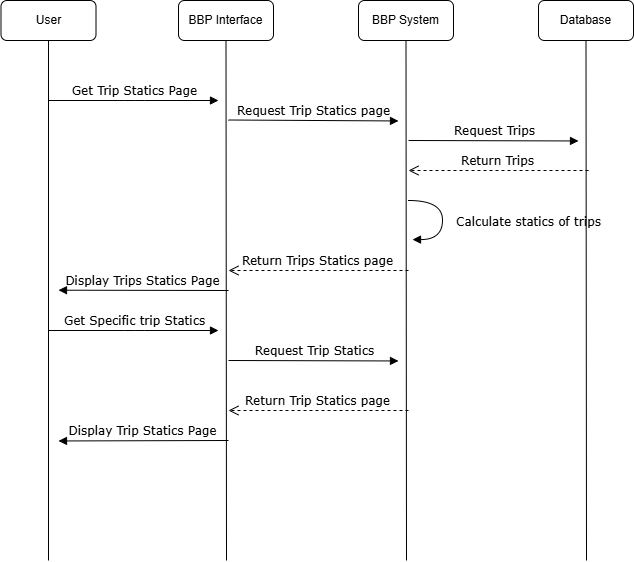
\includegraphics[width=1\linewidth]{Images/Diagrams/Sequence_ViewStatistics.png}
        \caption{Sequence Diagram for View Trip Statistics}
        \label{fig:view_statistics_seqd}%
    \end{center}
\end{figure}

\subsubsection*{UC\cuc . Check Review}
\begin{center}
    \begin{longtable}{|l|p{0.75\linewidth}|}
        \hline
        \textbf{Actor}            & User (Registered or Non-Registered) \\
        \hline
        \textbf{Entry Conditions} & 
        \begin{itemize}
            \item User has access to BBP platform
            \item Path exists with at least one review
        \end{itemize} \\
        \hline
        \textbf{Event Flow}       & 
        \begin{enumerate}
            \item User accesses path details interface
            \item User selects a path to view
            \item BBP displays path information
            \item User selects "View Reviews" option
            \item BBP retrieves all reviews for the path
            \item BBP displays reviews with:
            \begin{itemize}
                \item Reviewer username
                \item Rating given
                \item Written comment
                \item Date of review
                \item Path status reported at time of review
            \end{itemize}
            \item BBP shows reviews sorted by:
            \begin{itemize}
                \item Most recent first (default)
                \item Highest rating
                \item Lowest rating
            \end{itemize}
            \item User can filter reviews by:
            \begin{itemize}
                \item Date range
                \item Rating range
                \item Path status
            \end{itemize}
            \item User reads reviews to inform their decision
        \end{enumerate} \\
        \hline
        \textbf{Exit Conditions}   & 
        \begin{itemize}
            \item User has viewed reviews for the path
            \item User can make informed decision based on community feedback
        \end{itemize} \\
        \hline
        \textbf{Exceptions}       & 
        \begin{enumerate}
            \item \textbf{No reviews available:}
            \begin{itemize}
                \item Display message indicating no reviews yet
                \item Encourage user to add first review (if registered)
            \end{itemize}
            \item \textbf{Reviews loading error:}
            \begin{itemize}
                \item Display error message
                \item Provide retry option
            \end{itemize}
            \item \textbf{Network error:}
            \begin{itemize}
                \item Display cached reviews if available
                \item Notify user of connection issue
            \end{itemize}
        \end{enumerate} \\
        \hline
        \caption{Check Review Use Case.}
        \label{tab:check_review_use_case}
    \end{longtable}
\end{center}

\begin{figure}[H]
    \begin{center}
        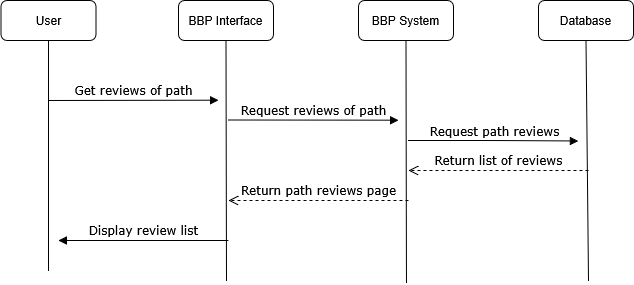
\includegraphics[width=1\linewidth]{Images/Diagrams/Sequence_CheckReview.png}
        \caption{Sequence Diagram for Check Review}
        \label{fig:check_review_seqd}%
    \end{center}
\end{figure}

\subsubsection*{UC\cuc . Merge Information from Multiple Users}
\begin{center}
    \begin{longtable}{|l|p{0.75\linewidth}|}
        \hline
        \textbf{Actor}            & System \\
        \hline
        \textbf{Entry Conditions} & 
        \begin{itemize}
            \item Multiple users have provided publishable information about the same path
            \item Path information exists from different sources
        \end{itemize} \\
        \hline
        \textbf{Event Flow}       & 
        \begin{enumerate}
            \item BBP detects multiple information sources for the same path
            \item BBP collects all publishable information about the path:
            \begin{itemize}
                \item Path status reports from different users
                \item Timestamps of each report
                \item Obstacle reports
            \end{itemize}
            \item BBP analyzes information freshness:
            \begin{itemize}
                \item Compares timestamps
                \item Identifies most recent information
            \end{itemize}
            \item BBP counts confirming data:
            \begin{itemize}
                \item Groups similar status reports
                \item Counts consensus for each status
            \end{itemize}
            \item BBP resolves conflicts:
            \begin{itemize}
                \item If consensus exists, uses majority status
                \item If no clear consensus, uses most recent information
            \end{itemize}
            \item BBP merges obstacle information:
            \begin{itemize}
                \item Combines obstacle reports
                \item Removes duplicates
                \item Prioritizes recent reports
            \end{itemize}
            \item BBP updates path status in database
        \end{enumerate} \\
        \hline
        \textbf{Exit Conditions}   & 
        \begin{itemize}
            \item Path information is merged and updated
            \item Merged information reflects consensus and freshness
        \end{itemize} \\
        \hline
        \textbf{Exceptions}       & 
        \begin{enumerate}
            \item \textbf{Conflicting information with equal weight:}
            \begin{itemize}
                \item Use most recent information
                \item Flag for manual review if needed
            \end{itemize}
            \item \textbf{No consensus found:}
            \begin{itemize}
                \item Maintain current status
                \item Wait for additional information
            \end{itemize}
            \item \textbf{Data inconsistency:}
            \begin{itemize}
                \item Log inconsistency for review
                \item Use most reliable source
            \end{itemize}
        \end{enumerate} \\
        \hline
        \caption{Merge Information from Multiple Users Use Case.}
        \label{tab:merge_information_use_case}
    \end{longtable}
\end{center}

\begin{figure}[H]
    \centering
    \vspace{-0.5cm}
    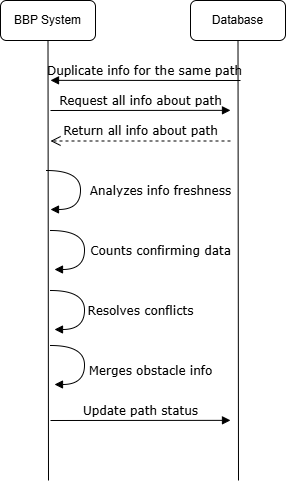
\includegraphics[width=0.35\linewidth]{Images/Diagrams/Sequence_MergeInformation.png}
    \vspace{-0.3cm}
    \caption{Sequence Diagram for Merge Information from Multiple Users}
    \label{fig:merge_information_seqd}%
    \vspace{-0.2cm}
\end{figure}

\newpage
\subsection{Mapping on Requirements}
\label{subsec:mapping_on_requirements}%

This section provides a comprehensive mapping between the identified use cases and the functional requirements they satisfy. This traceability matrix ensures that all functional requirements are covered by at least one use case and helps in understanding how the system's functionality is realized through user interactions.

\begin{table}[H]
    \centering
    \small
    \begin{longtable}{ |p{0.25\linewidth}|p{0.65\linewidth}| }
        \hline
        \textbf{Use Case} & \textbf{Functional Requirements} \\
        \hline
        UC1: User Registration & F1.1 (User account creation with validated email addresses) \\
        \hline
        UC2: Login & F1.2 (Secure login mechanisms protected by passwords) \\
        \hline
        UC3: Insert Path Information (Manual Mode) & F3.1 (Manual insertion of bike path information), F3.2 (Specify path status), F3.3 (Mark obstacles), F3.4 (Make path publishable), F3.5 (Store path information) \\
        \hline
        UC4: Insert Path Information (Automated Mode) & F4.1 (Automatic detection of cycling based on speed), F4.2 (Collect GPS information), F4.3 (Acquire accelerometer and gyroscope data), F4.4 (Present detected paths and obstacles), F4.5 (Allow user confirmation), F4.6 (Allow correction of false positives), F4.7 (Store confirmed path information) \\
        \hline
        UC5: Publish Path Information & F3.4 (Make path information publishable), F3.5 (Store path information) \\
        \hline
        UC6: Search and Visualize Paths Between Two Points & F5.1 (Specify origin and destination), F5.2 (Find available paths), F5.3 (Compute path score), F5.4 (Visualize paths on map) \\
        \hline
        UC7: Post Review & F3.2 (Specify path status), F3.3 (Mark obstacles) \\
        \hline
        UC8: Record Personal Trip & F2.1 (Manual trip recording), F2.4 (Store trip data), F2.5 (Calculate trip statistics), F2.6 (Retrieve meteorological information), F2.7 (View and manage recorded trips) \\
        \hline
        UC9: See Path Data & F5.1 (Specify origin and destination), F5.2 (Find available paths), F3.2 (Path status information), F3.3 (Obstacle information) \\
        \hline
        UC10: View Trip Statistics & F2.5 (Calculate trip statistics), F2.7 (View and manage recorded trips), F2.6 (Meteorological information integration) \\
        \hline
        UC11: Check Review & F3.2 (Path status information), F3.3 (Obstacle information) \\
        \hline
        UC12: Merge Information from Multiple Users & F6.1 (Collect publishable information from multiple users), F6.2 (Merge information considering freshness), F6.3 (Merge information considering confirming data), F6.4 (Resolve conflicts), F6.5 (Prioritize information based on recency and consensus) \\
        \hline
        \caption{Mapping of Use Cases to Functional Requirements}
        \label{tab:mapping_use_cases_requirements}
    \end{longtable}
    \normalsize
\end{table}

\newpage
\section{Performance Requirements}
\label{sec:performance_requirements}%

The main issue the system has to tackle when booting is loading the nearby map and paths. Another main aspect is loading all data from the user, their past trips, reviews, statistics, etc. However, these data can be retrieved quickly and BBP should not encounter any trouble running on almost any machine.


\newpage
\section{Design constraints}
\label{sec:design_constraints}%


\subsection{Design Constraints}
\label{subsec:design_constraints}%

\subsubsection*{Standards Compliance}
\raggedright
GDPR: BBP follows the European guidelines stated in the General Data Protection Regulation when managing the user's personal data.

ISO/IEC 27001: The system is prepared to manage any risk and security issues according to the software lifecycle management standard.

\subsubsection*{Development standards}
ISO/IEC 12207: The system shall apply the best practices across all relevant software life-cycle processes, including requirements analysis, design, implementation, verification, validation, deployment, operation, maintenance, and disposal.

\subsubsection*{Development Constraints}
\begin{itemize}
    \item \textbf{Mobile-First Architecture:} 
    The system will be accessible exclusively via native mobile applications for iOS and Android, designed to run on mobile devices with appropriate sensor access. The backend services will run on servers to support the mobile applications.
    \item \textbf{Mobile-Optimized Design:} 
    The platform must be optimized for mobile devices, ensuring an optimal user experience on smartphones with varying screen sizes and orientations. The interface is designed specifically for touch interactions and mobile device constraints.
    \item \textbf{Modular Components:} 
    The architecture will be modular, facilitating easier debugging, testing, and future enhancements by breaking functionality into independent, reusable components.
    \item \textbf{API-First Approach:} 
    Development will follow an API-first methodology, prioritizing a well-documented API layer that enables easy integration with external systems and scalability.
    \item \textbf{Sensor Access:} 
    Mobile applications must request and handle sensor permissions (GPS, accelerometer, gyroscope) appropriately according to iOS and Android platform guidelines.
    \item \textbf{Battery Optimization:} 
    Automatic trip recording must be optimized to minimize battery consumption on mobile devices.
\end{itemize}

\subsubsection*{Hardware Limitations}
\begin{itemize}
    \item \textbf{Mobile Device Sensors:} 
    System functionality depends on availability and accuracy of mobile device sensors (GPS, accelerometer, gyroscope). Performance may vary based on device capabilities.
    \item \textbf{Network Connectivity:} 
    Some features require internet connectivity. The system should handle offline scenarios gracefully with local data storage and synchronization.
    \item \textbf{Storage Limitations:} 
    Mobile devices have limited storage. The system should implement efficient data management and caching strategies.
\end{itemize}

\newpage
\section{Software System Attributes}
\label{sec:software_system_attributes}%

\subsubsection*{Reliability}
The system must ensure correct error handling and data processing and validation to ensure data integrity during trip, path and review management.

\subsubsection*{Availability}
The main services of BBP should have a fair amount of redundancy and failover mechanisms to prevent critical errors in the application. The system must also be prepared for cases when some services are unavailable, for example not showing the weather if the API is unavailable or downloading the map and some paths in case connection is lost.

\subsubsection*{Security}
Safe authentication system and secure password management, to protect user data and location information.

\subsubsection*{Maintainability}
The system shall implement a modular design for scalability, testing, maintainability and reusability. A correct version control protocol must be used and the documentation of said code has to be correct and up to date.

\subsubsection*{Portability}
The system should be functional in all mobile devices, easily updated and portable when new models or interfaces come up.
